\section{Introduction}



\begin{frame}{Research Objective}
\begin{itemize} 
    \item Different advanced GAN architectures are introduced to generate the future probability distribution of a financial time series given the previous history. 
    \vspace{5mm}
    \item The proposed GAN architectures are evaluated over Black-Scholes and Heston trajectories by using different statistical metrics
\end{itemize}
\end{frame}



\begin{frame}{Generative Adversarial Networks}
\begin{figure}[H]
    \centering
    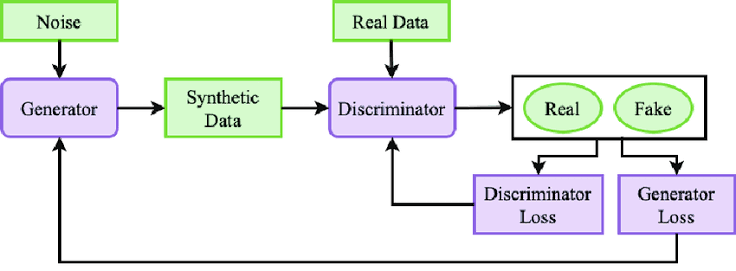
\includegraphics[scale=0.4]{images/gan_architecture.png}
\end{figure}
\begin{equation}
\min_G \max_D V(D,G) = \mathbb{E}_{x \sim p_{\mathrm{data}}(x)}\left[\log D(x|c)\right] + \mathbb{E}_{z \sim p_z(z)}\left[\log\left(1-D(G(z|c))\right)\right]
\end{equation}


\begin{equation}
\text{Generator Loss }\rightarrow \min_G V(D,G) = \mathbb{E}_{z \sim p_z(z)}\left[\log\left(1-D(G(z|c))\right)\right]
\end{equation}

This has been proved in the original GAN paper \cite{background:gan} to be equivalent to minimizing the Jensen-Shannon divergence between the real and generated data distributions.

\end{frame}





\begin{frame}{Wasserstein GAN}
    
The primal definition of the Wasserstein-1 distance 
for two probability distributions, $\mathbb{P}_r$ (real) and $\mathbb{P}_g$ (generated) is given 
by:
\begin{equation*}
    W(\mathbb{P}_r, \mathbb{P}_g) = \inf_{\pi \in \Pi(\mathbb{P}_r, \mathbb{P}_g)} \mathbb{E}_{(x, y) \sim \pi} [\|x - y\|]
\end{equation*}
where $\Pi(\mathbb{P}_r, \mathbb{P}_g)$ denotes the set of all joint distributions $\pi(x, y)$ with marginals $\mathbb{P}_r$ and $\mathbb{P}_g$.\\
\vspace{1cm}
CWGAN models rely on the Kantorovich-Rubinstein duality version (\cite{intro:duality}), which
transforms the constrained minimization over transport plans into a maximization over a
set of 1-Lipschitz continuous functions (the critic).

\begin{equation}
\min_G \max_D V(D,G) = \mathbb{E}_{x \sim p_{data}}[D(x \mid c)] 
- \mathbb{E}_{z \sim p_z}[D(G(z \mid c))]
+ \lambda GP
\end{equation}

with $GP$ the gradient penalty term that enforces the 1-Lipschitz constraint on the critic network.
\end{frame}
    


\begin{frame}{GAN architecture for time series probability forecasting}
   
To generate the future probability distribution of a time series $c = x_0, x_1, \ldots, x_t$, the following steps are taken:
\begin{enumerate}
    \item Train generator and discriminator using the CGAN or CWGAN loss function using $c_{[t_0, t]}$ as condition and $x_{t+1}$ as target.
    \item The generator is ran multiple times using the same trajectory $c$ but perturbated noise vector $z$ obtaining an empirical distribution.
\end{enumerate}

\begin{figure}[H]
    \centering
    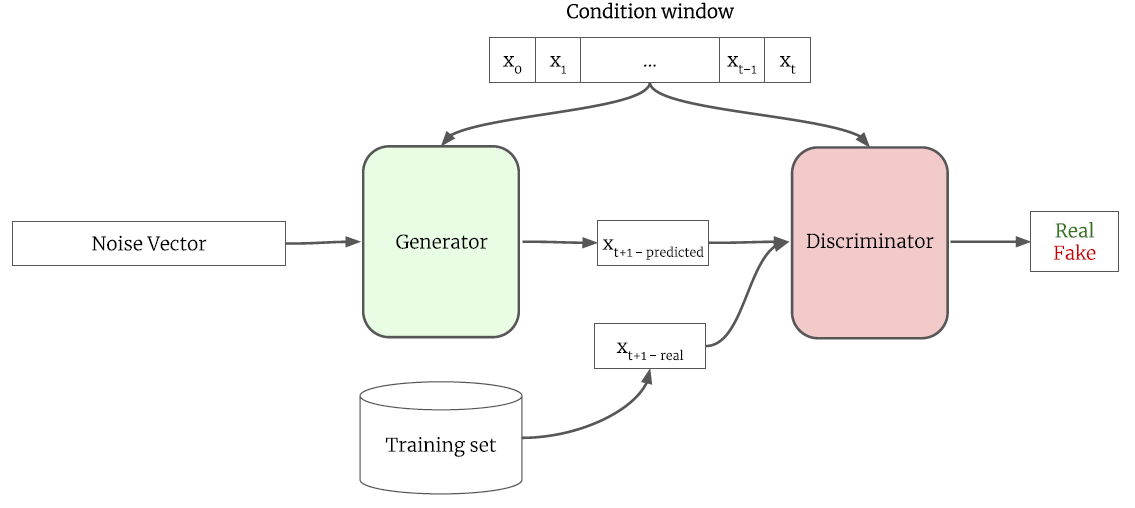
\includegraphics[scale=0.4]{images/forgan.png}
\end{figure}

\end{frame}


\begin{frame}{GAN architecture for time series probability forecasting}
\begin{columns}[c]

    \begin{column}{0.38\textwidth}

        \textbf{Generator}

        \vspace{0.1cm}

        It receives:
        \begin{itemize}
            \item conditioning information $c$ processed by a RNN that outputs a hidden state $h$
            \item latent noise $z$
            \item $z$ and $h$ are concatenated and processed by a FFN and outputs the next time step $x_{t+1}$
        \end{itemize}


        \textbf{Discriminator}

        \vspace{0.1cm}

        It receives the concatenated $(c, x_{t+1})$ 
        which is processed by a RNN. The hidden state $h$ is then processed by a FFN to output 
        the probability/score of the sample being real or fake.

    \end{column}

    \begin{column}{0.58\textwidth}

        \centering
        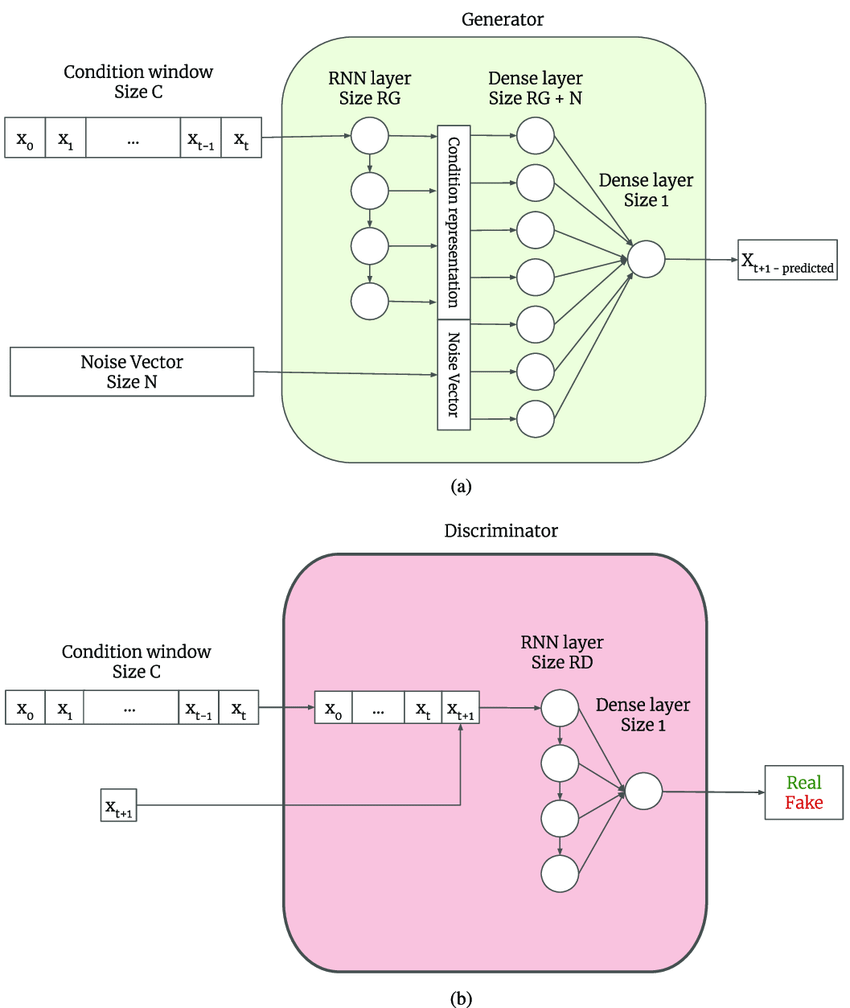
\includegraphics[height=0.82\textheight]{images/forgan_rnn.png}

    \end{column}

\end{columns}
\end{frame}


\begin{frame}{Realized volatility estimator}
Before computing the RV estimator a winsorization procedure is applied to each estimator component.
The proposed estimator is composed by 2 parts: 
\begin{itemize}
    \item The intraday price variation $\hat{RV_t} = \frac{PK_t + GK_t + RS_t}{3}$
    \item The overnight price variation $j_t^2 = (ln(O_t) - ln(C_{t-1}))^2$
\end{itemize}

Finally, the Realized Volatility estimator $RV_t = w_1 j_t^2 + w_2 \hat{RV_t}$ is obtained from the following minimization problem:
\begin{equation}
  \label{eq:opt_rv}
  \begin{aligned}
    &\textit{min}_{\omega \in \Omega}  \operatorname{VAR}[RV_t(\omega)] \\
    \textbf{is solved by: } & w_1^* = (1-\gamma)\frac{\mu_0}{\mu_1} \text{ and } w_2^* = \gamma\frac{\mu_0}{\mu_2}
  \end{aligned}
\end{equation}
 Where 
 \begin{itemize}
    \item $\gamma = \frac{\mu_2^2 \eta_1^2 - \mu_1 \mu_2 \eta_{12}}{\mu_2^2 \eta_1^2 + \mu_1^2 \eta_2^2 - 2\mu_1 \mu_2 \eta_{12}}$
    \item $\eta_2^2 = VAR[\hat{RV_t}]$
    \item $\eta_{12} = COV[\hat{RV_t}, j_t^2]$
    \item $\mu_0 = VAR[r_t]$
    \item $\mu_1 = \bar{j_t^2}$
    \item $\mu_2 = \bar{RV_t}$ 
 \end{itemize}
    
\end{frame}













